\documentclass[svgnames]{beamer}
\mode<presentation>
\usefonttheme{serif}
\usecolortheme{dove}
\useinnertheme{rounded}
\useoutertheme{smoothbars}
\setbeamercolor{item projected}{fg=black}

%\sloppy
\usepackage[english]{babel}
\usepackage[latin1]{inputenc}
\usepackage{times}
\usepackage{amsthm,amssymb,amsmath,graphicx}
\usepackage{color}
\usepackage{gastex}

\newcommand{\set}[1]{\{ #1 \}}
\newcommand{\PSPACE}{\mathrm{PSPACE}}
\newcommand{\QBF}{\mathrm{QBF}}
\newcommand{\NP}{\mathrm{NP}}
\newcommand{\Poly}{\mathrm{P}}


\title{The surprizing complexity of\\
generalized reachability games}
\author{\underline{Nathana\"el Fijalkow} \inst{1,2} \& Florian Horn \inst{1}}
\institute{LIAFA \\ CNRS \& Universit� Denis Diderot - Paris 7, France \\
\textbf{florian.horn@liafa.jussieu.fr}
\and \'ENS Cachan \\ \'Ecole Normale Sup�rieure de Cachan, France \\
\textbf{nathanael.fijalkow@gmail.com}}
\date{September 20th, 2010}
\subtitle{GAMES'2010 workshop}


\AtBeginSection[]
{
  \begin{frame}<beamer>{Outline}
    \tableofcontents[currentsection,currentsubsection]
  \end{frame}
}
\AtBeginSubsection[]
{
  \begin{frame}<beamer>{Outline}
    \tableofcontents[currentsection,currentsubsection]
  \end{frame}
}

\begin{document}

\begin{frame}
  \titlepage
\end{frame}

\section{Generalized reachability games}
\subsection{Games}

\begin{frame}{Players}
Two players: \textbf{Eve} and \textbf{Adam}.
\begin{center}
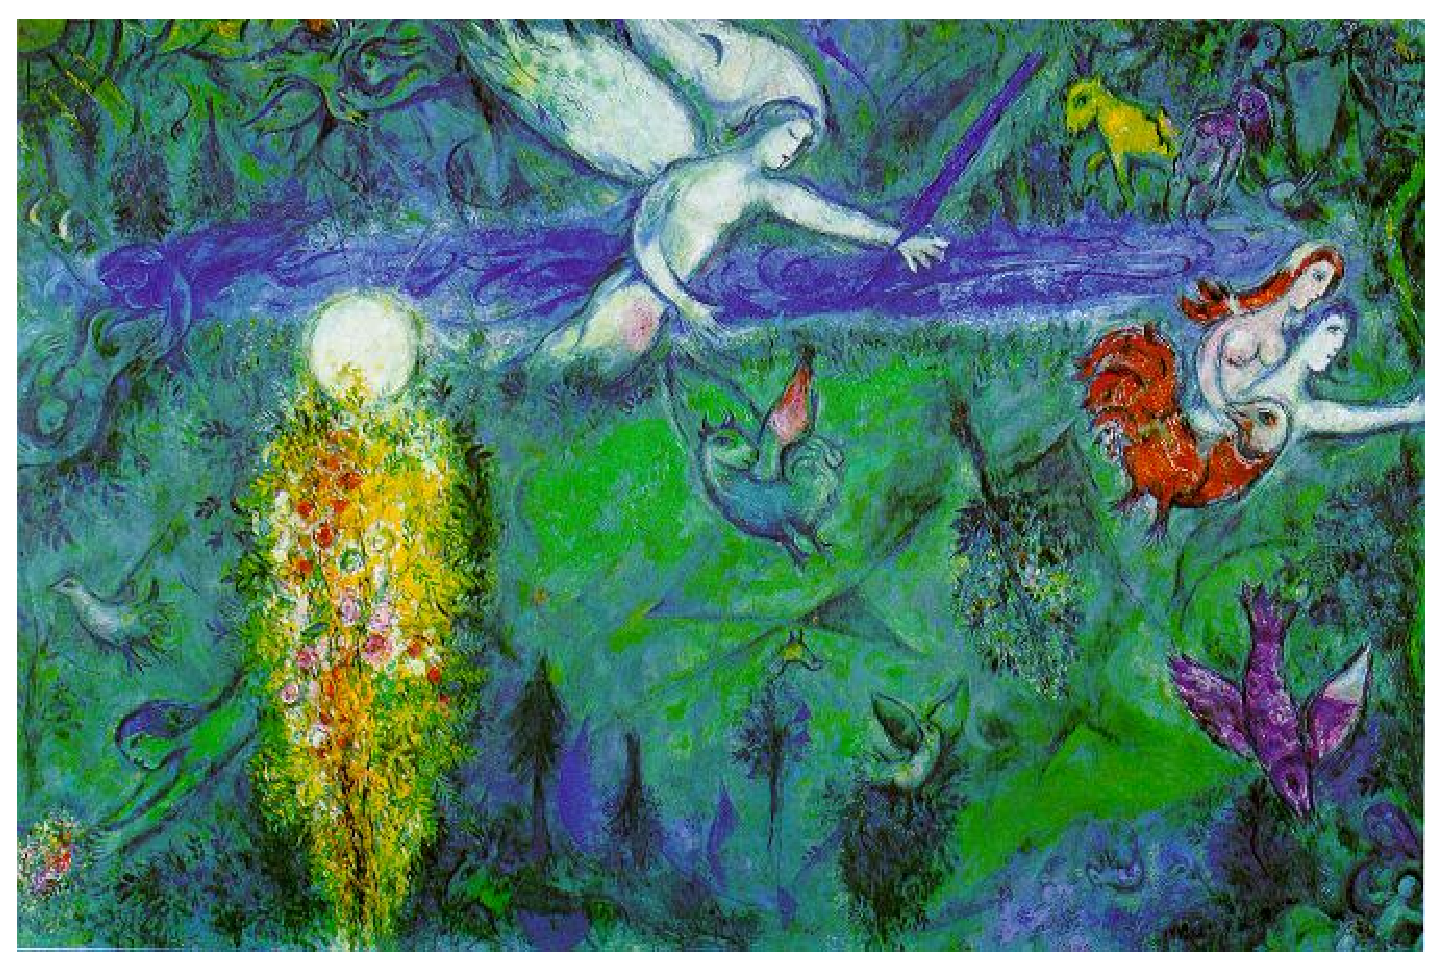
\includegraphics[scale=0.4]{Eve_and_Adam.eps}
\end{center}
\end{frame}

\begin{frame}{Playing}
\begin{center}
\begin{picture}(100,50)(0,0)
	\gasset{Nw=8,Nh=8}
	
  	\node(1)(60,30){}
  	\rpnode[polyangle=45](2)(50,15)(4,5){}
  	\node(3)(40,30){}
  	\rpnode[polyangle=45](4)(50,50)(4,5){}
  	\rpnode[polyangle=45](5)(50,0)(4,5){}
  	\node(6)(80,30){}
  	\node(7)(20,30){}

  	\drawedge(1,2){}
  	\drawedge(1,4){}
  	\drawedge(2,3){}
  	\drawedge(2,5){}
  	\drawedge(3,1){}
  	\drawedge[curvedepth=-5](3,5){}
  	\drawedge[curvedepth=10](4,6){}
  	\drawedge[curvedepth=-10](4,7){}
  	\drawedge[curvedepth=10](5,7){}
  	\drawedge(6,4){}
  	\drawedge(7,4){}
  	\drawedge[curvedepth=10](6,5){}
  	\drawedge[curvedepth=-5](5,1){}
  	\drawedge(7,3){}
	\drawloop[loopangle=90](4){}

\only<3>{\drawedge[AHLength=3,AHlength=4,linecolor=red,linewidth=0.7](1,2){}}
\only<5>{\drawedge[AHLength=3,AHlength=4,linecolor=red,linewidth=0.7](2,3){}}

\only<2,3>{\node[fillcolor=magenta,Nw=4,Nh=4](pebble)(60,30){}} %pebble on 1
\only<4,5>{\node[fillcolor=magenta,Nw=4,Nh=4](pebble)(50,15){}} %pebble on 2
\only<6>{\node[fillcolor=magenta,Nw=4,Nh=4](pebble)(40,30){}} %pebble on 3
\end{picture}
\end{center}
\end{frame}

\subsection{Reachability}

\begin{frame}{Solving reachability objectives}
\begin{center}
\begin{picture}(100,50)(0,0)
	\gasset{Nw=8,Nh=8}

	\put(0,50){Given {\color{red}{$F$}} $\subseteq Q$}
  	\node(1)(60,30){}
  	\rpnode[polyangle=45](2)(50,15)(4,5){}
  	\node(3)(40,30){}
  	\rpnode[polyangle=45](4)(50,50)(4,5){}
  	\rpnode[polyangle=45](5)(50,0)(4,5){}
  	\node(6)(80,30){}
  	\node(7)(20,30){}

  	\drawedge(1,2){}
  	\drawedge(1,4){}
  	\drawedge(2,3){}
  	\drawedge(2,5){}
  	\drawedge(3,1){}
  	\drawedge[curvedepth=-5](3,5){}
  	\drawedge[curvedepth=10](4,6){}
  	\drawedge[curvedepth=-10](4,7){}
  	\drawedge[curvedepth=10](5,7){}
  	\drawedge(6,4){}
  	\drawedge(7,4){}
  	\drawedge[curvedepth=10](6,5){}
  	\drawedge[curvedepth=-5](5,1){}
  	\drawedge(7,3){}
	\drawloop[loopangle=90](4){}
	
	\node[fillcolor=red](pebble)(60,30){$0$}
  	\rpnode[fillcolor=red,polyangle=45](2)(50,15)(4,5){$0$}
	\node[fillcolor=red](pebble)(40,30){$0$}

\only<2,3,4>{
	\node[fillcolor=red](pebble)(20,30){$1$}
}

\only<3,4>{
  	\rpnode[fillcolor=red,polyangle=45](2)(50,0)(4,5){$2$}
}

\only<4>{
  	\node[fillcolor=red](pebble)(80,30){$3$}
}
\end{picture}
\end{center}
\end{frame}

\subsection{Generalized}

\begin{frame}{Generalized reachability objectives}
\begin{itemize}
	\item Reachability objectives: given $F \subseteq Q$, reach at least one vertex in $F$;
	\item Generalized reachability objectives: given $F_1,F_2,\dots,F_p \subseteq Q$, reach at least one vertex in each $F_i$.
\end{itemize}
\end{frame}

\begin{frame}{Example}
\begin{center}
\begin{picture}(100,50)(0,0)
	\gasset{Nw=8,Nh=8}

	\put(0,60){Given {\color{red}{$F_1$}} and {\color{blue}{$F_2$}} $\subseteq Q$}

  	\node(1)(60,30){}
  	\rpnode[polyangle=45](2)(50,15)(4,5){}
  	\node(3)(40,30){}
  	\rpnode[polyangle=45](4)(50,50)(4,5){}
  	\rpnode[polyangle=45](5)(50,0)(4,5){}
  	\node(6)(80,30){}
  	\node(7)(20,30){}

  	\drawedge(1,4){}
  	\drawedge(3,2){}
  	\drawedge(2,5){}
  	\drawedge(6,1){}
  	\drawedge[curvedepth=3](2,1){}
  	\drawedge[curvedepth=3](1,2){}
  	\drawedge[curvedepth=5](5,3){}
  	\drawedge[curvedepth=10](4,6){}
  	\drawedge[curvedepth=-10](4,7){}
  	\drawedge[curvedepth=10](5,7){}
  	\drawedge[curvedepth=10](6,5){}
  	\drawedge[curvedepth=3](7,3){}
  	\drawedge[curvedepth=3](3,7){}
	\drawloop[loopangle=90](4){}
	
	\node[fillcolor=red](pebble)(60,30){}
  	\node[fillcolor=red](pebble)(40,30){}
	\node[fillcolor=blue](pebble)(20,30){}

\only<1>{\node[fillcolor=magenta,Nw=4,Nh=4](pebble)(80,30){}} %pebble
\only<2>{\node[fillcolor=magenta,Nw=4,Nh=4](pebble)(50,0){}} %pebble
\only<3>{\node[fillcolor=magenta,Nw=4,Nh=4](pebble)(20,30){}} %pebble
\only<4>{\node[fillcolor=magenta,Nw=4,Nh=4](pebble)(40,30){}} %pebble
\end{picture}
\end{center}
\end{frame}

\section{Complexity}
\subsection{$\PSPACE$-hardness: encoding $\QBF$}

\begin{frame}{Reduction from $\QBF$ to generalized reachability games}
$$\phi = \forall x\ \exists y\ \forall z\ \ \color{red}{(x \vee \neg y)} \ 
\color{black}{\wedge}\ \color{blue}{(\neg y \vee z)}$$
\pause
$$\color{red}{F_1 = \set{x,\neg y}} \hspace{2cm} \color{blue}{F_2 = \set{\neg y, z}}$$

\only<3>{Note that the number of literals in a clause is the size of the corresponding reachability set.}

\only<2>{
\begin{figure}
\begin{center}
\begin{picture}(80,20)(5,0)
	\gasset{Nw=7,Nh=7}
 
	\rpnode[polyangle=45,Nmarks=i](1)(0,10)(4,4){$\forall$}
	\node[linecolor=red](x)(15,20){$x$}
	\node(nx)(15,0){$\neg x$}

	\drawedge(1,x){}
	\drawedge(1,nx){}

	\node(2)(30,10){$\exists$}
	\node(y)(45,20){$y$}
	\node[linecolor=red](ny)(45,0){$\neg y$}
	\rmark[linecolor=blue](ny)
	
	\drawedge(x,2){}
	\drawedge(nx,2){}
	\drawedge(2,y){}
	\drawedge(2,ny){}

	\rpnode[polyangle=45](3)(60,10)(4,4){$\forall$}
	\node[linecolor=blue](z)(75,20){$z$}
	\node(nz)(75,0){$\neg z$}

	\drawedge(y,3){}
	\drawedge(ny,3){}
	\drawedge(3,z){}
	\drawedge(3,nz){}

	\node(e)(90,10){}
	\drawedge(z,e){}
	\drawedge(nz,e){}
	\drawloop[loopangle=0](e){}
\end{picture}
\end{center}
\end{figure}}
\end{frame}

\begin{frame}{Results}
\begin{theorem}[Lower bounds for generalized reachability games]
\begin{itemize}
	\item Solving two players generalized reachability games is $\PSPACE$-hard;
	\item Solving one player (Eve) generalized reachability games is $\NP$-hard.
\end{itemize}
\end{theorem}
\pause
\vskip3ex
\only<2>{Special cases where reachability sets have size less than $3$ \textit{might} be easier\dots}
\end{frame}

\begin{frame}{An easier case}
\begin{lemma}[A polynomial special case]
Solving two players generalized reachability games where reachability sets are singletons is in $\Poly$.
\end{lemma}

\only<2>{Why bigger reachability sets is harder to handle?
\begin{center}
\begin{picture}(50,30)(0,5)
 	\gasset{Nw=7,Nh=7}
  
	\put(-25,30){\color{orange}{$F_1 = \set{v_1,u_1}$}}
	\put(-25,24){\color{blue}{$F_2 = \set{v_2,u_2}$}}

 	\rpnode[polyangle=45](1)(0,15)(4,5){start}

 	\node[fillcolor=orange](v1)(15,30){$v_1$}
 	\node[fillcolor=blue](v2)(15,0){$v_2$}
 
 	\drawedge(1,v1){}
 	\drawedge(1,v2){}

 	\node(m)(30,15){m}
 
 	\node[fillcolor=orange](u1)(45,30){$u_1$}
 	\node[fillcolor=blue](u2)(45,0){$u_2$}
 
 	\drawedge(v1,m){}
 	\drawedge(v2,m){}
 	\drawedge(m,u1){}
 	\drawedge(m,u2){}
 
 	\drawloop[loopangle=45](u1){}
 	\drawloop[loopangle=45](u2){}
\end{picture}
\end{center}
}
\pause
\vskip2ex
\only<3>{If reachability sets are singletons, then Eve can predict the objectives vertices appearance order.}
\end{frame}

\subsection{Memory requirements}

\begin{frame}{Exponential lower bound for Eve, reachability sets of size $2$}
%Let $F_i = \set{u_i,v_i}$ and $k = 2p$.
\begin{center}
\begin{picture}(60,70)(0,0)
 	\gasset{Nw=8,Nh=8}
  
 	\rpnode[polyangle=45](1)(10,70)(4,5){start}
 	\rpnode[fillcolor=orange,polyangle=45](v1)(0,55)(4,5){$v_1$}
 	\rpnode[fillcolor=blue,polyangle=45](v2)(20,55)(4,5){$v_2$}
 
 	\drawedge(1,v1){}
 	\drawedge(1,v2){}
 
 	\rpnode[fillcolor=green,polyangle=45](v3)(0,40)(4,5){$v_3$}
 	\rpnode[fillcolor=red,polyangle=45](v4)(20,40)(4,5){$v_4$}

	\node[linecolor=white](v5)(0,25){}
	\node[linecolor=white](v6)(20,25){}
	
 	\drawedge(v1,v3){}
 	\drawedge(v1,v4){}
 	\drawedge(v2,v3){}
 	\drawedge(v2,v4){}
 	\drawedge(v3,v5){}
 	\drawedge(v4,v6){}
 
 	\gasset{Nw=.8,Nh=.8,Nfill=y}
 	\node(p1)(10,30){}
 	\node(p2)(10,26){}
 	\node(p3)(10,22){}
 	\gasset{Nw=8,Nh=8,Nfill=n}
 
 	\rpnode[polyangle=45,Nadjust=w,fillcolor=pink](v2p-1)(0,15)(4,6){$v_{2p-1}$}
 	\rpnode[polyangle=45,Nadjust=w,fillcolor=magenta](v2p)(20,15)(4,6){$v_{2p}$}
 
 	\node(2)(50,10){m}
 	\drawedge[curvedepth=-12](v2p-1,2){}
 	\drawedge[curvedepth=-8](v2p,2){}
 
 	\node[fillcolor=orange](u1)(40,25){$u_1$}
 	\node[fillcolor=blue](u2)(60,25){$u_2$}
 
 	\drawedge(2,u1){}
 	\drawedge(2,u2){}
 
 	\node[fillcolor=green](u3)(40,40){$u_3$}
 	\node[fillcolor=red](u4)(60,40){$u_4$}

	\node[linecolor=white](u5)(40,55){}
	\node[linecolor=white](u6)(60,55){}
 
 	\drawedge(u1,u3){}
 	\drawedge(u1,u4){}
 	\drawedge(u2,u3){}
 	\drawedge(u2,u4){}
 	\drawedge(u3,u5){}
 	\drawedge(u4,u6){}
 
 	\gasset{Nw=.8,Nh=.8,Nfill=y}
 	\node(p1)(50,46){}
 	\node(p2)(50,50){}
 	\node(p3)(50,54){}
 	\gasset{Nw=9,Nh=8,Nfill=n}
 
 	\node[fillcolor=pink](u2p-1)(40,60){$u_{2p-1}$}
 	\node[fillcolor=magenta](u2p)(60,60){$u_{2p}$}
 
 	\drawloop[loopangle=90](u2p-1){}
 	\drawloop[loopangle=90](u2p){}
\end{picture}
\end{center}
\end{frame}

\begin{frame}{Florian's piece of art; exponential lower bound for Eve}

\begin{figure}
\begin{center}
\unitlength = 3.5mm
\begin{picture}(16,24)(-8,-16)
	\gasset{Nw=2,Nh=2,Nmr=2}

	\node[Nmr=0](coeur)(0,0){}
	\node[linecolor=white](racine)(1,-13){}
					
	\drawedge[curvedepth=1.4](racine,coeur){}

	\gasset{Nw=1.5,Nh=1.5,Nmr=1.2}
	
	\node(a1)(0.59,6.05){}
	\node[fillcolor=blue](b1)(2.52,5.54){}
	\node(c1)(1.16,4.35){}
	\node[fillcolor=green,Nw=1.5,Nh=1.5](c12)(1.16,4.35){}
	\node[fillcolor=orange,Nw=1.1,Nh=1.1](c13)(1.16,4.35){}
	\node[fillcolor=red,Nw=.7,Nh=.7](c14)(1.16,4.35){}
	\node[fillcolor=pink,Nw=.3,Nh=.3](c15)(1.16,4.35){}

	\drawedge[curvedepth=.7](coeur,a1){}
	\drawedge[curvedepth=2](a1,b1){}
	\drawedge[curvedepth=.7](b1,coeur){}
	\drawedge[curvedepth=.4](a1,c1){}
	\drawloop[loopangle=255,loopdiam=1](c1){}

	\node(a2)(5.86,1.62){}
	\node[fillcolor=green](b2)(6.07,-0.37){}
	\node(c2)(4.48,0.47){}
	\node[fillcolor=blue,Nw=1.5,Nh=1.5](c22)(4.48,0.47){}
	\node[fillcolor=orange,Nw=1.1,Nh=1.1](c23)(4.48,0.47){}
	\node[fillcolor=red,Nw=.7,Nh=.7](c24)(4.48,0.47){}
	\node[fillcolor=pink,Nw=.3,Nh=.3](c25)(4.48,0.47){}

	\drawedge[curvedepth=.7](coeur,a2){}
	\drawedge[curvedepth=2](a2,b2){}
	\drawedge[curvedepth=.7](b2,coeur){}
	\drawedge[curvedepth=.4](a2,c2){}
	\drawloop[loopangle=186,loopdiam=1](c2){}

	\node(a3)(3.61,-4.89){}
	\node[fillcolor=orange](b3)(1.83,-5.80){}
	\node(c3)(2.04,-4.01){}
	\node[fillcolor=blue,Nw=1.5,Nh=1.5](c12)(2.04,-4.01){}
	\node[fillcolor=green,Nw=1.1,Nh=1.1](c13)(2.04,-4.01){}
	\node[fillcolor=red,Nw=.7,Nh=.7](c14)(2.04,-4.01){}
	\node[fillcolor=pink,Nw=.3,Nh=.3](c15)(2.04,-4.01){}

	\drawedge[curvedepth=.7](coeur,a3){}
	\drawedge[curvedepth=2](a3,b3){}
	\drawedge[curvedepth=.7](b3,coeur){}
	\drawedge[curvedepth=.4](a3,c3){}
	\drawloop[loopangle=117,loopdiam=1](c3){}

	\node(ai)(-4.49,-4.11){}
	\node[fillcolor=red](bi)(-5.58,-2.43){}
	\node(ci)(-3.77,-2.45){}
	\node[fillcolor=blue,Nw=1.5,Nh=1.5](ci2)(-3.77,-2.45){}
	\node[fillcolor=green,Nw=1.1,Nh=1.1](ci3)(-3.77,-2.45){}
	\node[fillcolor=orange,Nw=.7,Nh=.7](ci4)(-3.77,-2.45){}
	\node[fillcolor=pink,Nw=.3,Nh=.3](ci5)(-3.77,-2.45){}

	\drawedge[curvedepth=.7](coeur,ai){}
	\drawedge[curvedepth=2](ai,bi){}
	\drawedge[curvedepth=.7](bi,coeur){}
	\drawedge[curvedepth=.4](ai,ci){}
	\drawloop[loopangle=33,loopdiam=1](ci){}

	\node(ak)(-5.44,2.72){}
	\node[fillcolor=pink](bk)(-4.27,4.34){}
	\node(ck)(-3.64,2.65){}
	\node[fillcolor=blue,Nw=1.5,Nh=1.5](ck2)(-3.64,2.65){}
	\node[fillcolor=green,Nw=1.1,Nh=1.1](ck3)(-3.64,2.65){}
	\node[fillcolor=orange,Nw=.7,Nh=.7](ck4)(-3.64,2.65){}
	\node[fillcolor=red,Nw=.3,Nh=.3](ck5)(-3.64,2.65){}

	\drawedge[curvedepth=.7](coeur,ak){}
	\drawedge[curvedepth=2](ak,bk){}
	\drawedge[curvedepth=.7](bk,coeur){}
	\drawedge[curvedepth=.4](ak,ck){}
	\drawloop[loopangle=324,loopdiam=1](ck){}
\end{picture}
\end{center}
\end{figure}

\end{frame}

\begin{frame}{Conclusion and further work}
\begin{itemize}
	\item Conjuntions of easy objectives may be way harder to solve;
	\item Open case: reachability sets of size $2$.
\end{itemize}
\end{frame}

\begin{frame}{The end.}
Thank for your attention!
\end{frame}

\end{document}